\documentclass{article}
\usepackage{xcolor}
\usepackage{titleps}
\usepackage[letterpaper, margin=0.95in]{geometry}
\usepackage{url}
\usepackage{amsmath}
\usepackage{amssymb}
\usepackage{wrapfig}
\usepackage{float}
\usepackage{mathtools}
\usepackage{enumitem}
\usepackage{tabu}
\usepackage{parskip}
\usepackage{natbib}
\usepackage{listings}

\usepackage[many]{tcolorbox}
\usepackage{minted}
\setminted[python]{
	% frame=single,
	% linenos,
    xleftmargin=0.475em,
    baselinestretch=1.2,
}
% https://tex.stackexchange.com/a/569249
\setcounter{secnumdepth}{5}
\setcounter{tocdepth}{5}
\makeatletter
\newcommand\subsubsubsection{\@startsection{paragraph}{4}{\z@}{-2.5ex\@plus -1ex \@minus -.25ex}{1.25ex \@plus .25ex}{\normalfont\normalsize\bfseries}}
\newcommand\subsubsubsubsection{\@startsection{subparagraph}{5}{\z@}{-2.5ex\@plus -1ex \@minus -.25ex}{1.25ex \@plus .25ex}{\normalfont\normalsize\bfseries}}
\makeatother

\usepackage{hyperref}
\usepackage[color=red]{todonotes}
\usepackage{forest}
\definecolor{light-yellow}{HTML}{FFE5CC}

\newpagestyle{ruled}
{\sethead{CMU 16-831}{Introduction to Robot Learning }{Fall 2024}\headrule
  \setfoot{}{}{}}
\pagestyle{ruled}

\renewcommand\makeheadrule{\color{black}\rule[-.75\baselineskip]{\linewidth}{0.4pt}}
\renewcommand*\footnoterule{}

\newtcolorbox[]{answer}[1][]{
    % breakable,
    enhanced,
    nobeforeafter,
    colback=white,
    title=Your Answer,
    sidebyside align=top,
    box align=top,
    #1
}



\begin{document}

\lstset{basicstyle = \ttfamily,columns=fullflexible,
backgroundcolor = \color{light-yellow}
}

\begin{centering}
    {\Large Assignment 2: Policy Gradient} \\
    \vspace{.25cm}
    % \textbf{Due September 13, 11:59 pm} \\
\end{centering}
\vspace{0.25cm}

\textbf{Andrew ID:} \texttt{yulongl} \\
\textbf{Collaborators:} \texttt{None} \\
\textbf{NOTE:} Please do \textbf{NOT} change the sizes of the answer blocks or plots.

\setcounter{section}{4}
\section{Small-Scale Experiments}

\subsection{Experiment 1 (Cartpole) -- \lbrack25 points total\rbrack}

\subsubsection{Configurations}
\begin{answer}[title=Q5.1.1,height=6cm,width=\linewidth]
% TODO
\begin{minted}
[framesep=2mm, fontsize=\scriptsize, breaklines]
{bash}
python rob831/scripts/run_hw2.py --env_name CartPole-v0 -n 100 -b 1000 \
    -dsa --exp_name q1_sb_no_rtg_dsa

python rob831/scripts/run_hw2.py --env_name CartPole-v0 -n 100 -b 1000 \
    -rtg -dsa --exp_name q1_sb_rtg_dsa

python rob831/scripts/run_hw2.py --env_name CartPole-v0 -n 100 -b 1000 \
    -rtg --exp_name q1_sb_rtg_na

python rob831/scripts/run_hw2.py --env_name CartPole-v0 -n 100 -b 5000 \
    -dsa --exp_name q1_lb_no_rtg_dsa

python rob831/scripts/run_hw2.py --env_name CartPole-v0 -n 100 -b 5000 \
    -rtg -dsa --exp_name q1_lb_rtg_dsa

python rob831/scripts/run_hw2.py --env_name CartPole-v0 -n 100 -b 5000 \
    -rtg --exp_name q1_lb_rtg_na
\end{minted}
\end{answer}

\subsubsection{Plots}

\subsubsubsection{Small batch -- \lbrack5 points\rbrack}
\begin{answer}[title=Q5.1.2.1,height=9.5cm,width=\linewidth]
% TODO
\centering
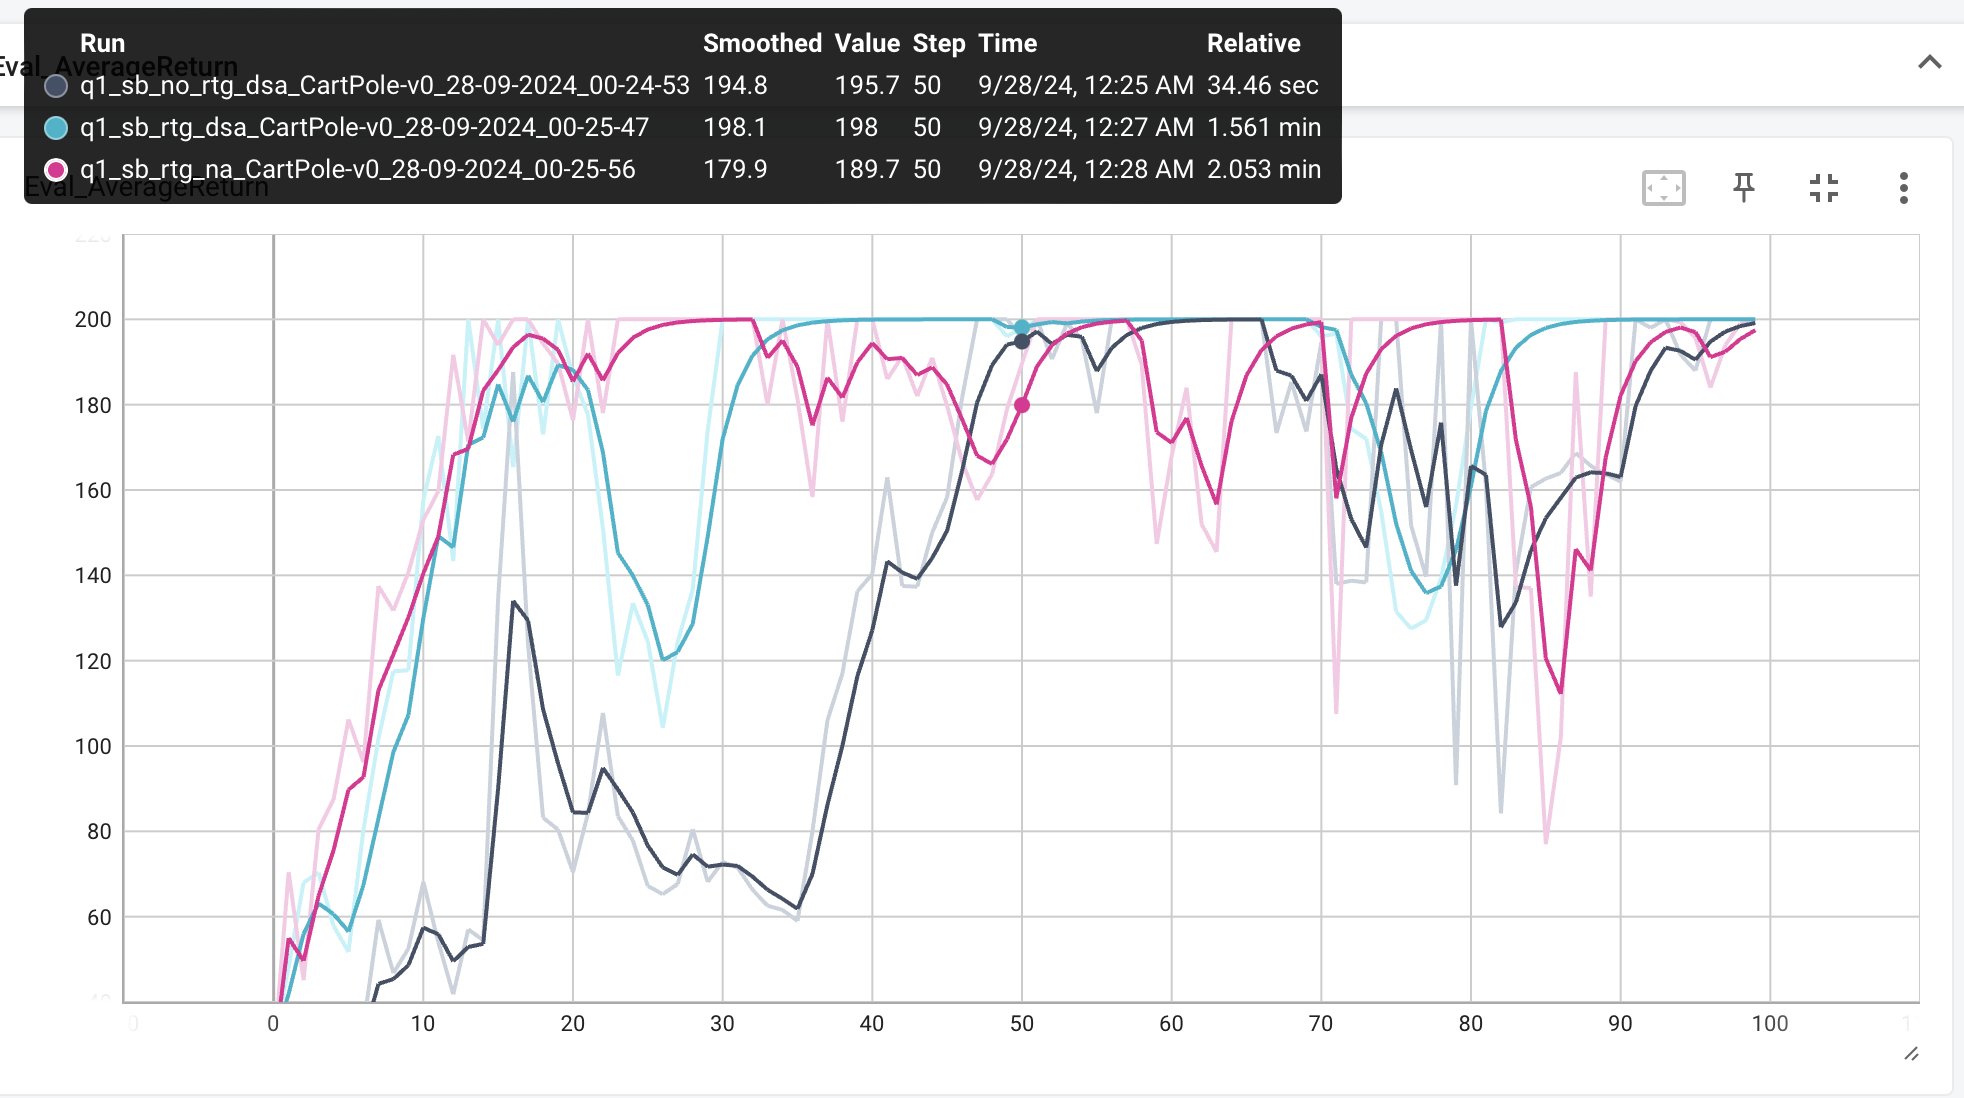
\includegraphics[height=8cm]{figures/q1_sb.png}
\end{answer}

\subsubsubsection{Large batch -- \lbrack5 points\rbrack}
\begin{answer}[title=Q5.1.2.2,height=9.5cm,width=\linewidth]
% TODO
\centering
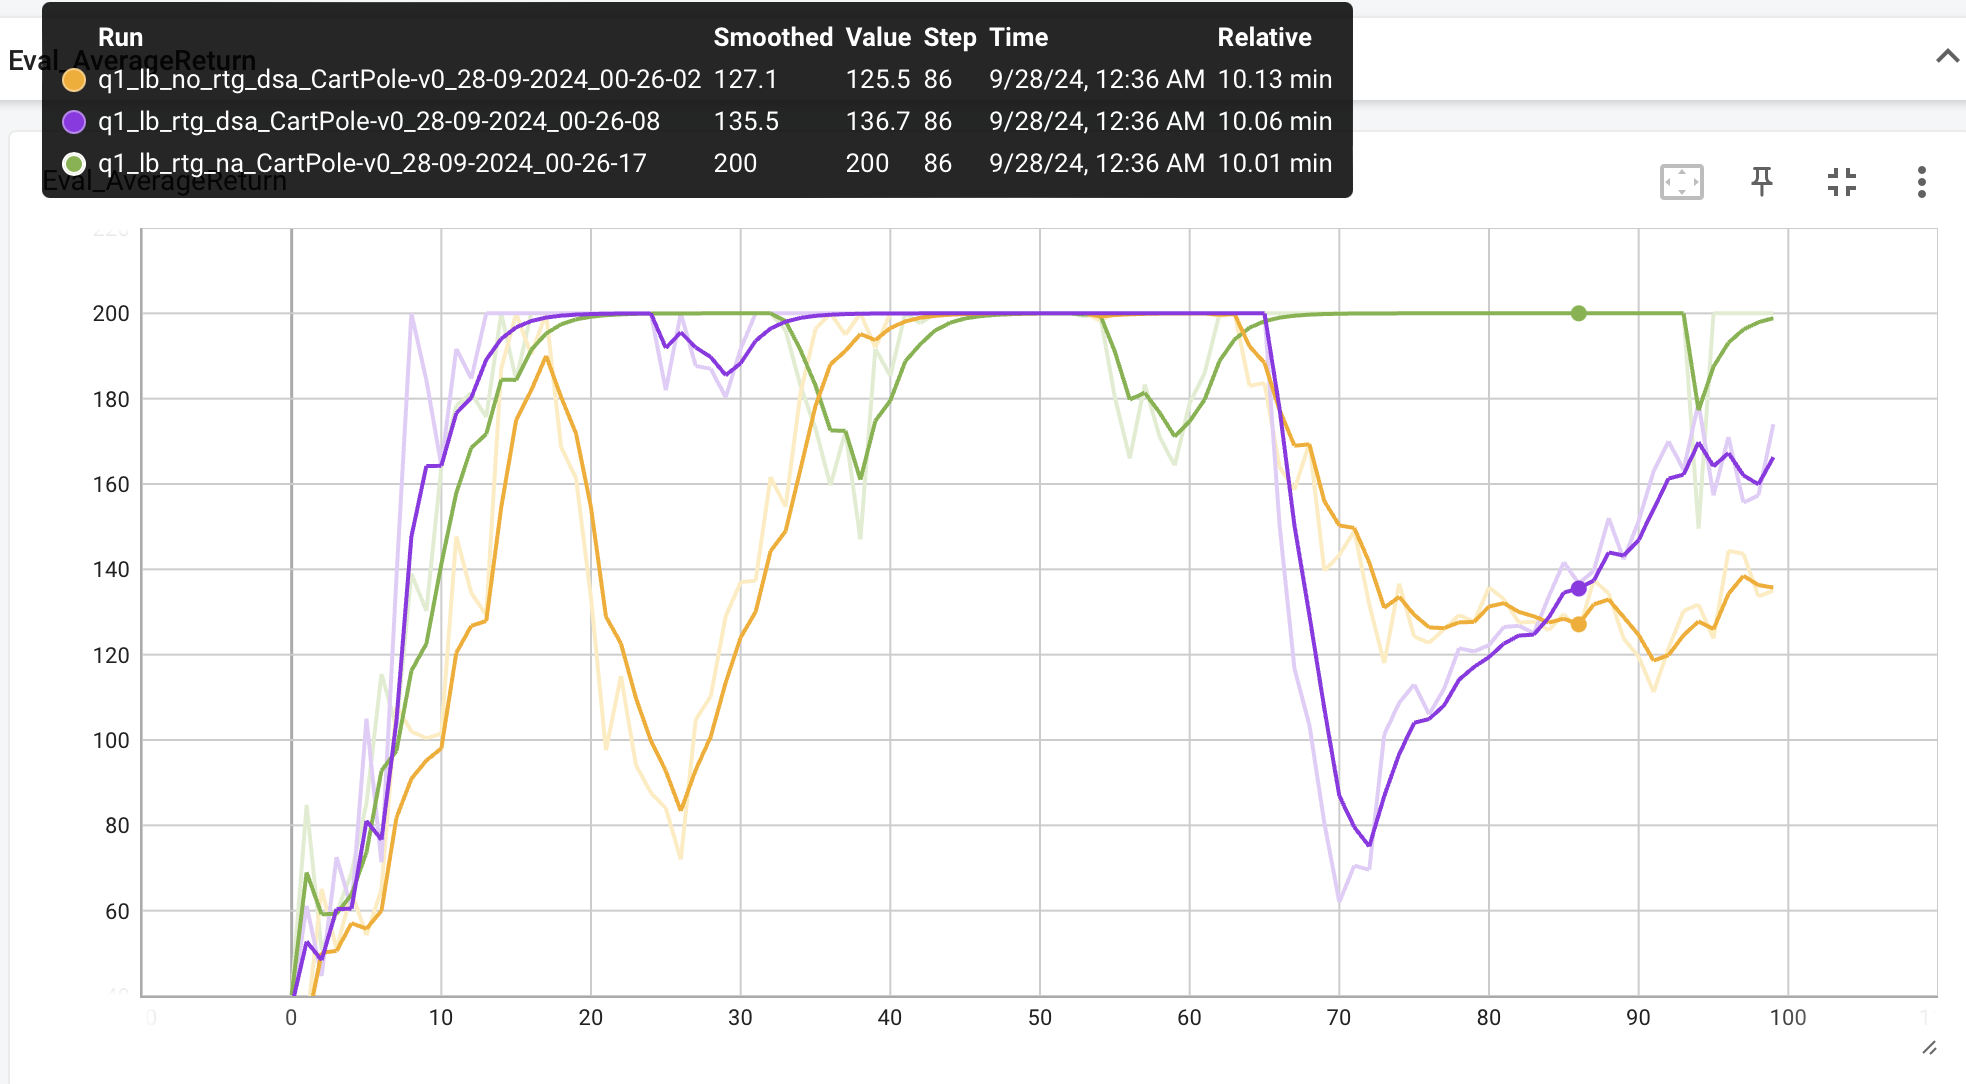
\includegraphics[height=8cm]{figures/q1_lb.png}
\end{answer}

\subsubsection{Analysis}

\subsubsubsection{Value estimator -- \lbrack5 points\rbrack}
\begin{answer}[title=Q5.1.3.1,height=4cm,width=\linewidth]
% TODO
Without advantage standardization, the reward to go value estimator performs better and more stable than the trajectory-centric value estimator for both the small batch and the large batch.
\end{answer}

\subsubsubsection{Advantage standardization -- \lbrack5 points\rbrack}
\begin{answer}[title=Q5.1.3.2,height=4cm,width=\linewidth]
% TODO
Based on my experiments, it is unclear whether advantage standardization is helpful for the Cartpole task. For both small batch and large batch, the performance with advantage standardization has higher variance.
\end{answer}

\subsubsubsection{Batch size -- \lbrack5 points\rbrack}
\begin{answer}[title=Q5.1.3.3,height=4cm,width=\linewidth]
% TODO
Based on my experiments, it is unclear whether batch size is helpful for the Cartpole task. For both small batch and large batch, the return s converge to around 200 at around 15 iterations. Large batch even seems to have higher variance. However, this might due to the randomness in the experiments.
\end{answer}

\subsection{Experiment 2 (InvertedPendulum) -- \lbrack15 points total\rbrack}

\subsubsection{Configurations -- \lbrack5 points\rbrack}
\begin{answer}[title=Q5.2.1,height=10cm,width=\linewidth]
% TODO
\begin{minted}
[framesep=2mm, fontsize=\scriptsize, breaklines]
{bash}

for b in 1000 5000 10000
do
  for lr in 0.005 0.01 0.02 0.03
  do
    CUDA_VISIBLE_DEVICES=1 python rob831/scripts/run_hw2.py --env_name InvertedPendulum-v4 \
    --ep_len 1000 --discount 0.9 -n 100 -l 2 -s 64 -b $b -lr $lr -rtg \
    --exp_name q2_b${b}_r${lr}
  done
done
\end{minted}
\end{answer}

\subsubsection{smallest \textbf{b*} and largest \textbf{r*} (same run) -- \lbrack5 points\rbrack}
\begin{answer}[title=Q5.2.2,height=4cm,width=\linewidth]
% TODO
b* = 1000, r* = 0.01
\end{answer}

\subsubsection{Plot -- \lbrack5 points\rbrack}
\begin{answer}[title=Q5.2.3,height=10cm,width=\linewidth]
% TODO
\centering
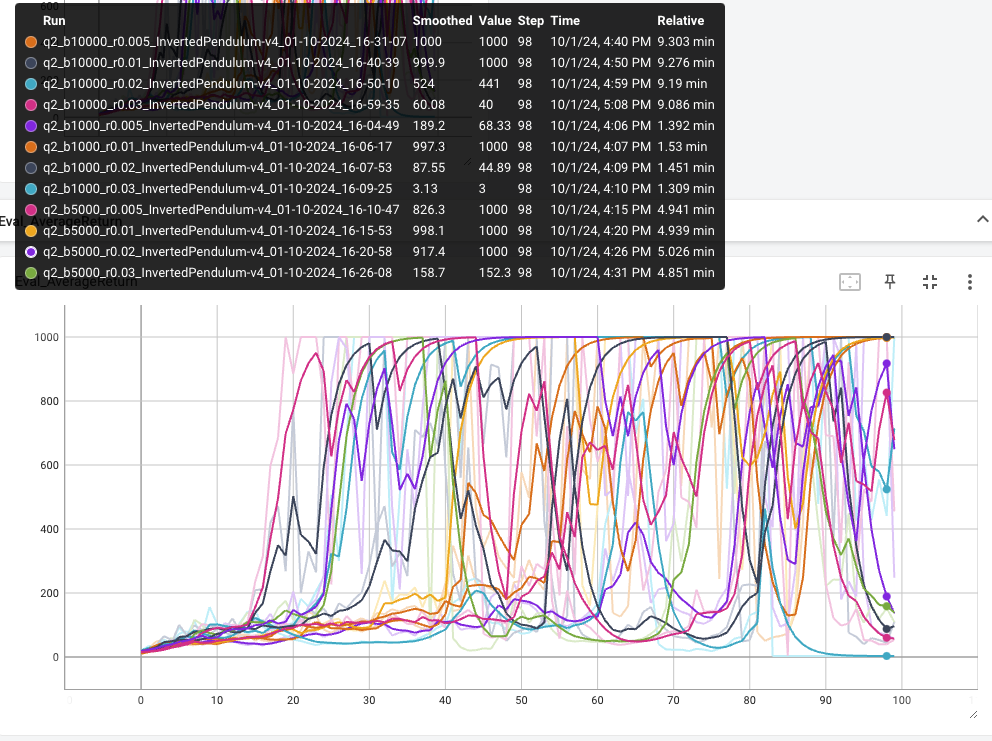
\includegraphics[height=8cm]{figures/q2.png}
\end{answer}

\setcounter{section}{6}
\section{More Complex Experiments}

\subsection{Experiment 3 (LunarLander) -- \lbrack10 points total\rbrack}

\subsubsection{Configurations}
\begin{answer}[title=Q7.1.1,height=6cm,width=\linewidth]
\begin{minted}
[framesep=2mm, fontsize=\scriptsize, breaklines]
{bash}
python rob831/scripts/run_hw2.py \
    --env_name LunarLanderContinuous-v4 --ep_len 1000
    --discount 0.99 -n 100 -l 2 -s 64 -b 10000 -lr 0.005 \
    --reward_to_go --nn_baseline --exp_name q3_b10000_r0.005
\end{minted}
\end{answer}

\subsubsection{Plot -- \lbrack10 points\rbrack}
\begin{answer}[title=Q7.1.2,height=10cm,width=\linewidth]
% TODO
\centering
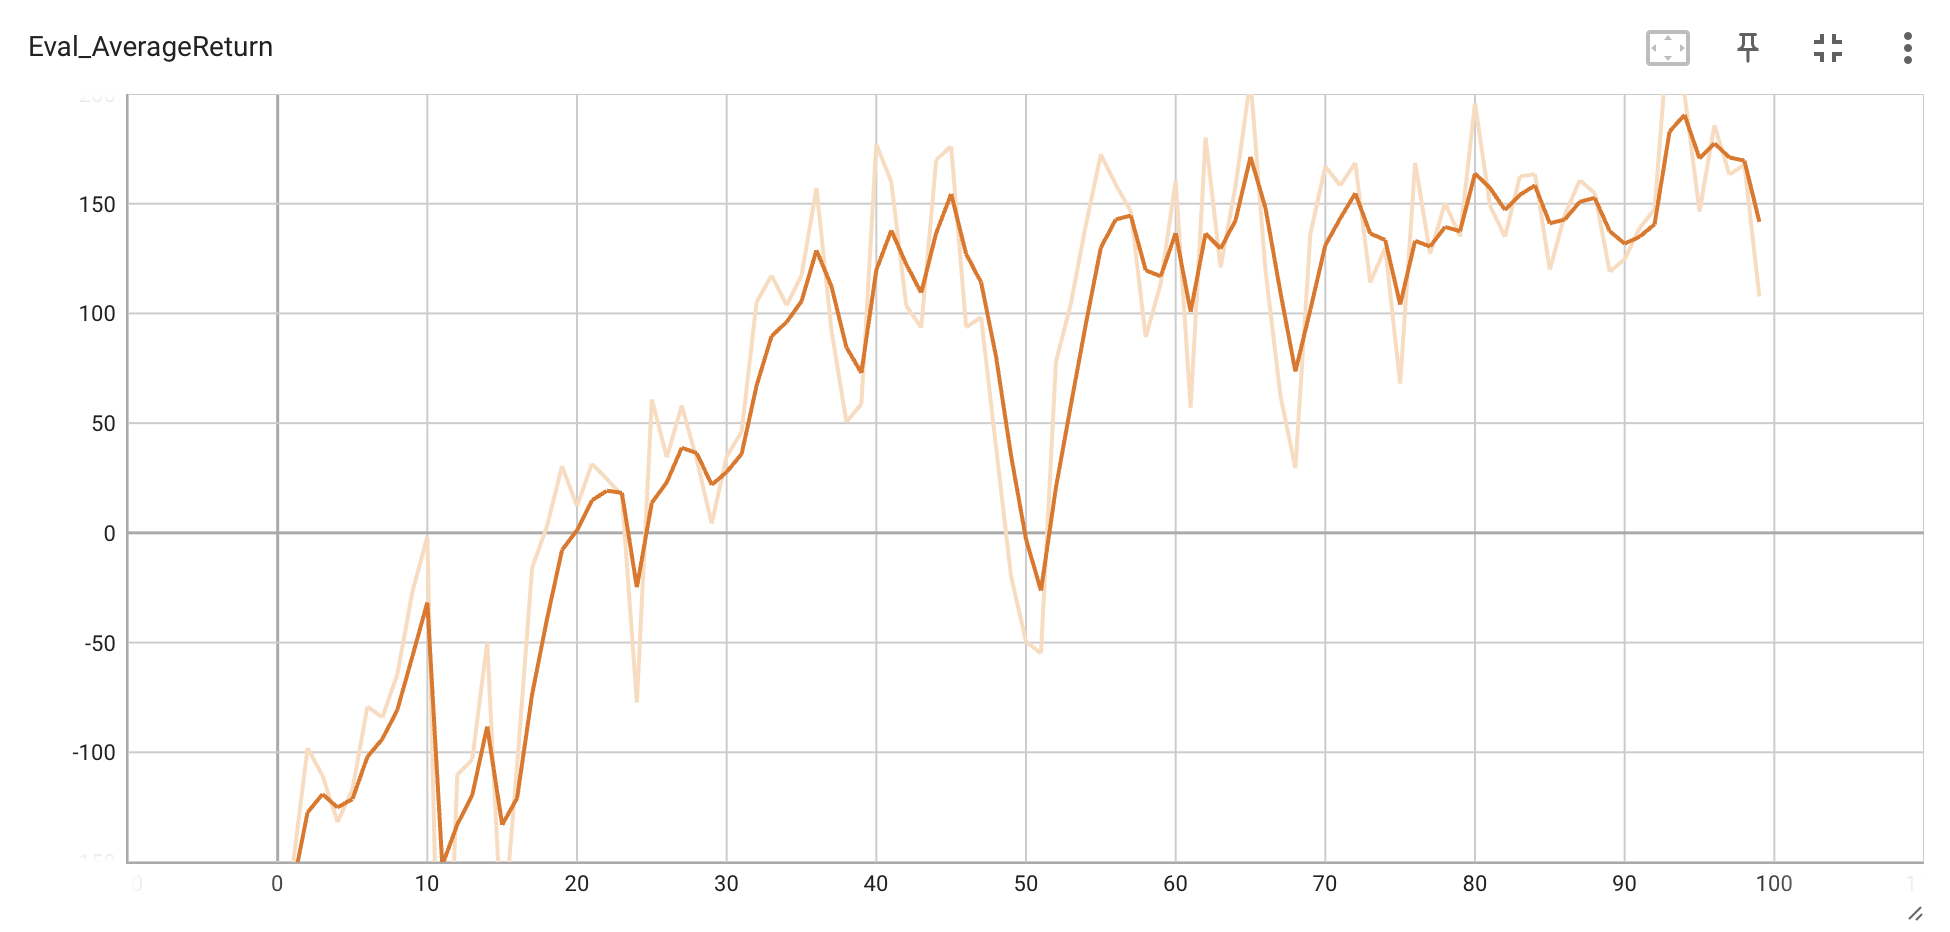
\includegraphics[height=8cm]{figures/q3.png}
\end{answer}

\subsection{Experiment 4 (HalfCheetah) -- \lbrack30 points\rbrack}

\subsubsection{Configurations}
\begin{answer}[title=Q7.2.1,height=10cm,width=\linewidth]
\begin{minted}
[framesep=2mm, fontsize=\scriptsize, breaklines, escapeinside=||, mathescape=true]
{python}
python rob831/scripts/run_hw2.py --env_name HalfCheetah-v4 --ep_len 150 \
    --discount 0.95 -n 100 -l 2 -s 32 -b 10000 -lr 0.02 \
    --exp_name q4_search_b10000_lr0.02
python rob831/scripts/run_hw2.py --env_name HalfCheetah-v4 --ep_len 150 \
    --discount 0.95 -n 100 -l 2 -s 32 -b 10000 -lr 0.02 -rtg \
    --exp_name q4_search_b10000_lr0.02_rtg
python rob831/scripts/run_hw2.py --env_name HalfCheetah-v4 --ep_len 150 \
    --discount 0.95 -n 100 -l 2 -s 32 -b 10000 -lr 0.02 --nn_baseline \
    --exp_name q4_search_b10000_lr0.02_nnbaseline
python rob831/scripts/run_hw2.py --env_name HalfCheetah-v4 --ep_len 150 \
    --discount 0.95 -n 100 -l 2 -s 32 -b 10000 -lr 0.02 -rtg --nn_baseline \
    --exp_name q4_search_b10000_lr0.02_rtg_nnbaseline
\end{minted}
\end{answer}

\subsubsection{Plot -- \lbrack10 points\rbrack}
\begin{answer}[title=Q7.2.2,height=10cm,width=\linewidth]
% TODO
\centering
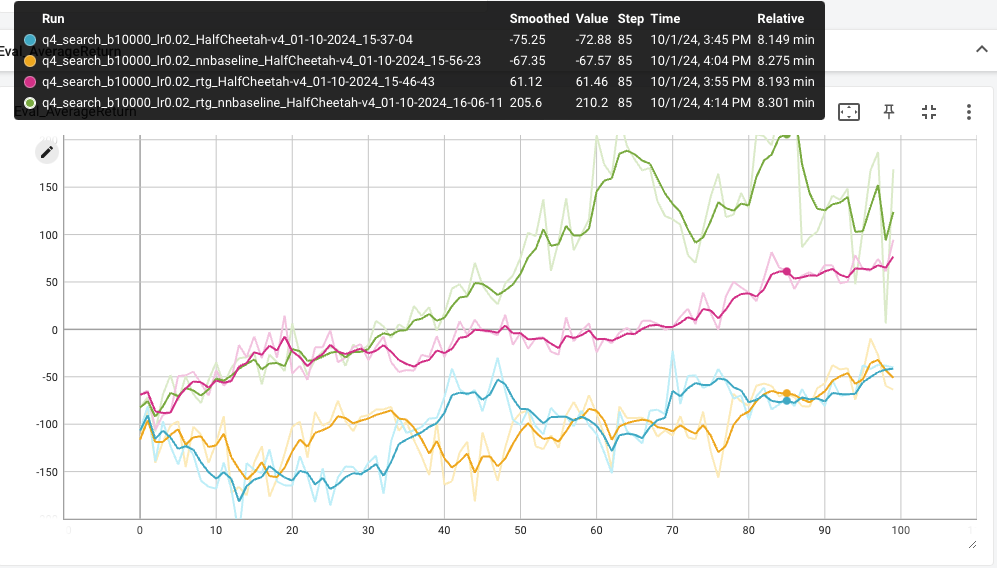
\includegraphics[height=8cm]{figures/q41.png}
\end{answer}

\subsubsection{(Optional) Optimal b* and r* -- \lbrack3 points\rbrack}
\begin{answer}[title=Q7.2.3,height=4cm,width=\linewidth]
% TODO
I found that $b^* = 10000$ and $r^* = 0.02$ for the HalfCheetah task.
\end{answer}

\subsubsection{(Optional) Plot -- \lbrack10 points\rbrack}
\begin{answer}[title=Q7.2.4,height=10cm,width=\linewidth]
% TODO
\centering
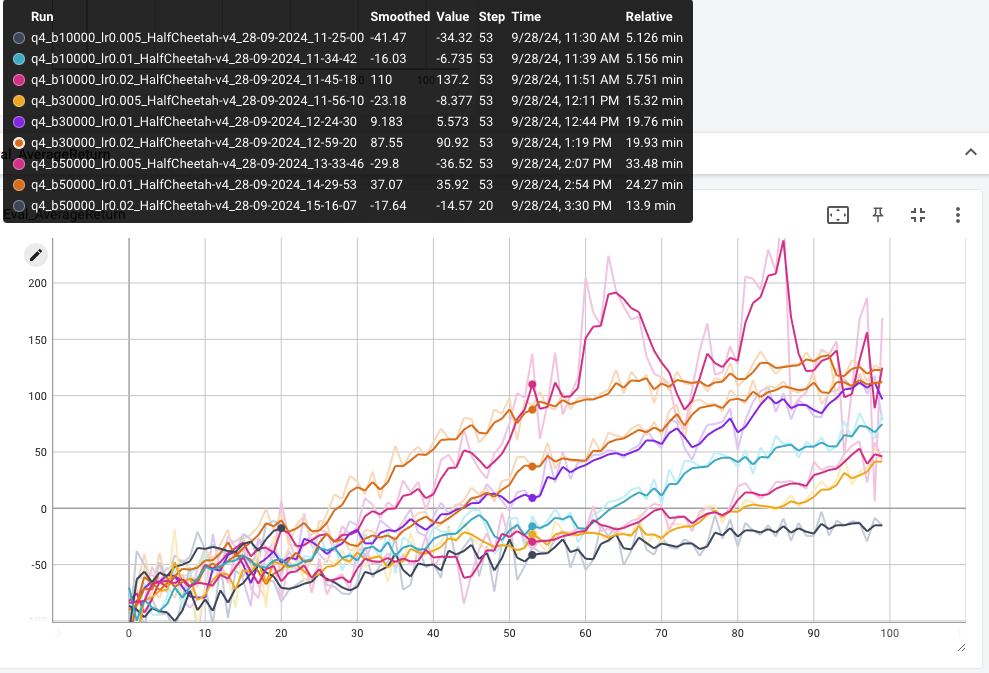
\includegraphics[height=8cm]{figures/q42.png}
\end{answer}

\subsubsection{(Optional) Describe how b* and r* affect task performance -- \lbrack7 points\rbrack}
\begin{answer}[title=Q7.2.5,height=4cm,width=\linewidth]
% TODO
With larger b*, the training is more stable and variance is reduced. With larger r*, the agent learns faster. In fact, with b*=30000 and r*=0.02, the agents achieves slightly inferior performance to b*=10000 and r*=0.02, but the training is more stable. With more iterations, the performance of b*=30000 and r*=0.02 is likely to be better. However, for 100 iterations, the performance of b*=10000 and r*=0.02 is the most optimal.
\end{answer}

\subsubsection{(Optional) Configurations with optimal b* and r* -- \lbrack3 points\rbrack}
\begin{answer}[title=Q7.2.6,height=6cm,width=\linewidth]
% TODO
\begin{minted}
    [framesep=2mm, fontsize=\scriptsize, breaklines, escapeinside=||, mathescape=true]
    {python}
    python rob831/scripts/run_hw2.py --env_name HalfCheetah-v4 --ep_len 150 \
        --discount 0.95 -n 100 -l 2 -s 32 -b 10000 -lr 0.02 \
        --exp_name q4_search_b10000_lr0.02
    python rob831/scripts/run_hw2.py --env_name HalfCheetah-v4 --ep_len 150 \
        --discount 0.95 -n 100 -l 2 -s 32 -b 10000 -lr 0.02 -rtg \
        --exp_name q4_search_b10000_lr0.02_rtg
    python rob831/scripts/run_hw2.py --env_name HalfCheetah-v4 --ep_len 150 \
        --discount 0.95 -n 100 -l 2 -s 32 -b 10000 -lr 0.02 --nn_baseline \
        --exp_name q4_search_b10000_lr0.02_nnbaseline
    python rob831/scripts/run_hw2.py --env_name HalfCheetah-v4 --ep_len 150 \
        --discount 0.95 -n 100 -l 2 -s 32 -b 10000 -lr 0.02 -rtg --nn_baseline \
        --exp_name q4_search_b10000_lr0.02_rtg_nnbaseline
\end{minted}
\end{answer}

\subsubsection{(Optional) Plot for four runs with optimal b* and r* -- \lbrack7 points\rbrack}
\begin{answer}[title=Q7.2.7,height=10cm,width=\linewidth]
% TODO
\centering
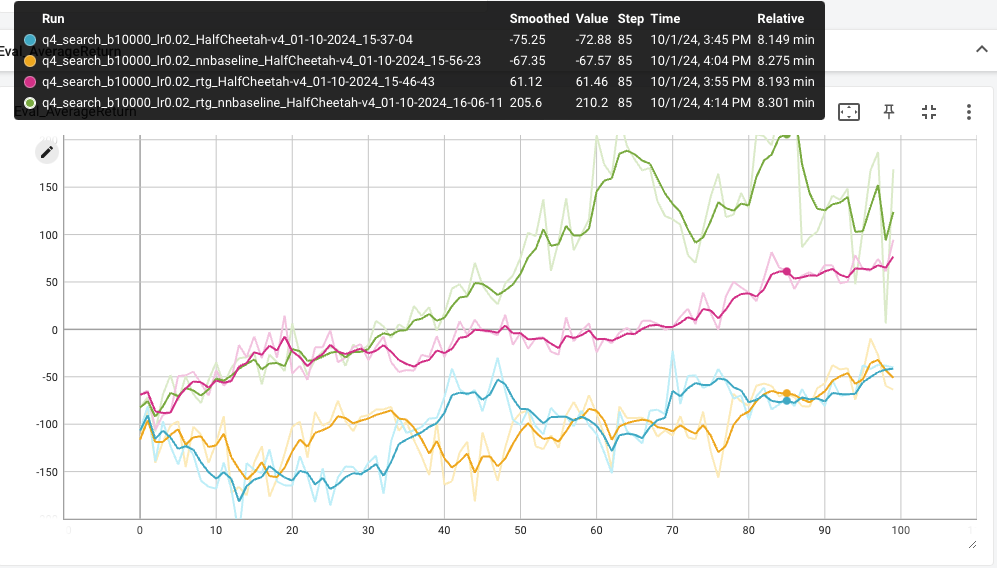
\includegraphics[height=8cm]{figures/q41.png}
\end{answer}

\section{Implementing Generalized Advantage Estimation}

\subsection{Experiment 5 (Hopper) -- \lbrack20 points\rbrack}

\subsubsection{Configurations}
\begin{answer}[title=Q8.1.1,height=4cm,width=\linewidth]
\begin{minted}
[framesep=2mm, fontsize=\scriptsize, breaklines, escapeinside=||, mathescape=true]
{python}
# $\lambda \in [0,0.95,0.99,1]$
python rob831/scripts/run_hw2.py \
    --env_name Hopper-v4 --ep_len 1000
    --discount 0.99 -n 300 -l 2 -s 32 -b 2000 -lr 0.001 \
    --reward_to_go --nn_baseline --action_noise_std 0.5 --gae_lambda <|$\lambda$|> \
    --exp_name q5_b2000_r0.001_lambda<|$\lambda$|>
\end{minted}
\end{answer}

\subsubsection{Plot -- \lbrack13 points\rbrack}
\begin{answer}[title=Q8.1.2,height=10cm,width=\linewidth]
% TODO
\centering
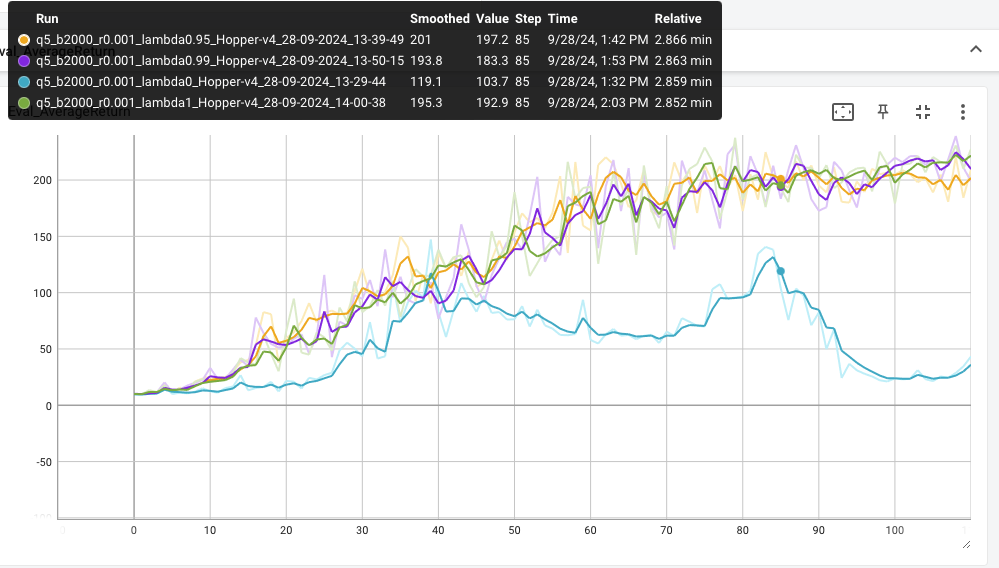
\includegraphics[height=8cm]{figures/q5.png}
\end{answer}

\subsubsection{Describe how $\lambda$ affects task performance -- \lbrack7 points\rbrack}
\begin{answer}[title=Q8.1.3,height=4cm,width=\linewidth]
% TODO
With $\lambda = 0$, the performance is the worst, and performance is similar for $\lambda = 0.95, 0.99, 1$. This shows that a baseline is needed to reduce variance and improve the performance.
\end{answer}

\clearpage

\section{Bonus! (optional)}

\subsection{Parallelization -- \lbrack15 points\rbrack}
\begin{answer}[title=Q9.1,height=4cm,width=\linewidth]
% TODO (optional)
Difference in training time: 5m25s vs 1m12s (8 threads)
\vspace{1.0cm}
\begin{minted}
[framesep=2mm, fontsize=\scriptsize, breaklines]
{bash}
time python rob831/scripts/run_hw2.py --env_name CartPole-v0 -n 100 -b 1000 -rtg -dsa --num_threads 1 --exp_name q6_1_thread;
time python rob831/scripts/run_hw2.py --env_name CartPole-v0 -n 100 -b 1000 -rtg -dsa --num_threads 8 --exp_name q6_8_threads;
\end{minted}
\end{answer}

\subsection{Multiple gradient steps -- \lbrack5 points\rbrack}
\begin{answer}[title=Q9.1,height=14cm,width=\linewidth]
% TODO (optional)
\centering
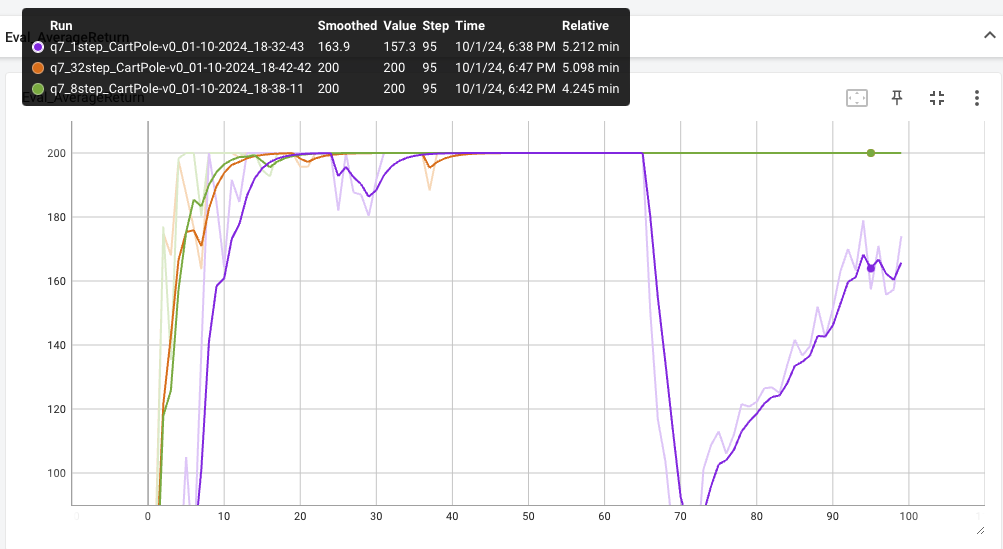
\includegraphics[height=8cm]{figures/q7.png}

\vspace{1.0cm}
\begin{minted}
[framesep=2mm, fontsize=\scriptsize, breaklines]
{bash}
python rob831/scripts/run_hw2.py --env_name CartPole-v0 -n 100 -b 5000 -rtg -dsa --num_agent_train_steps_per_iter 1 --exp_name q7_1step
python rob831/scripts/run_hw2.py --env_name CartPole-v0 -n 100 -b 5000 -rtg -dsa --num_agent_train_steps_per_iter 8 --exp_name q7_8step
python rob831/scripts/run_hw2.py --env_name CartPole-v0 -n 100 -b 5000 -rtg -dsa --num_agent_train_steps_per_iter 32 --exp_name q7_32step
\end{minted}

\end{answer}

\end{document}

